\documentclass[11pt]{article}
\usepackage[utf8]{inputenc}
\usepackage[T1]{fontenc}
\usepackage{fixltx2e}
\usepackage{graphicx}
\usepackage{longtable}
\usepackage{float}
\usepackage{wrapfig}
\usepackage{soul}
\usepackage{textcomp}
\usepackage{marvosym}
\usepackage{wasysym}
\usepackage{latexsym}
\usepackage{amssymb}
\usepackage{hyperref}
\tolerance=1000
\usepackage{fullpage}
\providecommand{\alert}[1]{\textbf{#1}}

\title{Report on Cyclotron Experiment}
\author{Craig Roy}
\date{\today}
\hypersetup{
  pdfkeywords={},
  pdfsubject={},
  pdfcreator={Emacs Org-mode version 7.9.3f}}

\begin{document}

\maketitle


\section*{Cyclotron}
\label{sec-1}
\subsection*{Description}
\label{sec-1-1}

This experiment simulates a kind of particle accelerator called a
cyclotron. A cyclotron operates by applying an alternating electric
field between two D-shaped metal structures referred to as
``Dees''. This causes a static particle between the Dees to enter one of
the Dees where it is then shielded from the electric field, but
exposed to a magnetic field within the Dee. This magnetic field
causes the particle's trajectory to rotate so that it then leaves the Dee and reenters the electric field, increasing its velocity and thus putting it in a wider and wider spiral until the particle exits the cyclotron entirely.

This experiment allows the user to observe the effects of adjusting
the frequency at which the electric field oscillates in the
cyclotron. It also allows the user to change the initial velocity of
the particle, the charge and the mass.
\subsection*{How to use it}
\label{sec-1-2}

Along the top of the simulation window, the editable fields for the
values of charge, x and y components of the velocity are shown, along
with the play/pause and reset buttons.
The cyclotron frequency is the field displayed at the bottom of the
window. A plot of the kinetic energy can be shown by clicking the
``Kinetic Energy Plot'' checkbox at the bottom of the screen.
\subsection*{How it works}
\label{sec-1-3}
\subsubsection*{Variables}
\label{sec-1-3-1}
\begin{itemize}

\item Var table
\label{sec-1-3-1-1}%
\begin{itemize}
\item \emph{b} is the magnetic field vector.
\item \emph{x, y} are the x and y positions of the particle.
\item \emph{vx, vy} are the velocity of the particle in the x and y directions respectively.
\item \emph{q} is the charge of the particle in the simulation. It is initially
  set to 1, so that the particle acts as a proton.
\item \emph{m} is the mass of the particle in the simulation.
\item \emph{t} is the time variable of the system.
\end{itemize}

\item Plotting
\label{sec-1-3-1-2}%
\begin{itemize}
\item \emph{ke} is the kinetic energy of the system, given by $ke = \frac{1}{2}mv^2$.
\item \emph{fx} is the force acting on the particle in the x direction due to
  the magnetic field.
\item \emph{fy} is the force acting on the particle in the y direction due to
  the magnetic field.
\item \emph{showPlot} is the variable behind the ``Kinetic Energy Plot'' checkbox.
\end{itemize}


\item E field
\label{sec-1-3-1-3}%
\begin{itemize}
\item \emph{e} is the electric field vector.
\item \emph{freq} is the frequency at which the electric field direction oscillates.
\item \emph{amp} is the magnitude of the electromagnetic field.
\end{itemize}


\item Semicircle
\label{sec-1-3-1-4}%
\begin{itemize}
\item \emph{semiCircX} is the array of points used to plot one of the Dees
  along the x-axis.
\item \emph{semiCircY} is the array of points used to plot one of the Dees
  along the y-axis.
\item \emph{r} is the radius of the semicircle.
\end{itemize}

\end{itemize} % ends low level
\subsubsection*{Initialisation}
\label{sec-1-3-2}

The initialisation section of the simulation is used to populate the
arrays of points which are used to plot the semicircle using the
custom method \emph{getX}.
\subsubsection*{Evolution}
\label{sec-1-3-3}

The evolution page sets up a couple of ODEs such that the rate and which \emph{x} and \emph{y} increase are equal to \emph{vx} and \emph{vy} respectively.

The rate at which \emph{vx} increases is proportional to the Lorentz force in the
x-direction. If the particle is in one of the Dees then the Lorentz
force is only affected by the magnetic field strength. If the particle
is between the Dees, the Lorentz force is only affected by the
electric field strength. The Lorentz force is calculated using the
custom functions \emph{calcForce} and \emph{eForce}. These values are then
divided by mass of the particle to find the acceleration from the
force.

The rate at which \emph{vy} increases is not affected by the electric field
strength, so it is calculated using \emph{calcForce} when the particle is
in one of the Dees.

The electric field vector \emph{e} is given by the cosine
function, \[ A\cdot\cos{f t} \] where \emph{A} is the variable \emph{amp} and
\emph{f} is the variable \emph{freq}.
\subsubsection*{Custom}
\label{sec-1-3-4}

\begin{itemize}
\item \emph{calcForce} takes arguments of the current x and y position and a
  velocity and returns the Lorentz force acting on the particle due to
  the magnetic field. It uses the function \emph{isInDee} to determine
  whether the particle is in one of the Dees. If the particle is not
  in one of the Dees, the \emph{calcForce} returns zero.
\item \emph{eForce} returns the Lorentz force acting on the particle due to the
  electric field. If the particle is not in the electric field,
  \emph{eForce} returns zero.
\item \emph{getX} is used to plot the Dees. Given a y-coordinate and the radius
  of the circle, it returns the corresponding x-coordinate.
\item \emph{isInDee} is used to determine whether the particle is in a Dee or
  not, by checking the x-coordinate and the y-coordinate.
\end{itemize}
\subsubsection*{Fixed Relations}
\label{sec-1-3-5}

The only fixed relation is to set the kinetic energy, \emph{ke} equal to $\frac{1}{2}mv^2$.
\subsubsection*{UI}
\label{sec-1-3-6}
\begin{itemize}

\item Top panel\\
\label{sec-1-3-6-1}%
The panel along the top consists of various fields and labels, as well
as the play/pause button and the reset button.

\item Drawing panel\\
\label{sec-1-3-6-2}%
This panel consists of the drawn part of the simulation. The
proton/electron particle in the system is represented by a 2dObject
called `particle'.
\begin{itemize}
\item \emph{rightDee} is a shape which is formed using the points in
  \emph{semiCircX} and \emph{semiCircY}. It is shifted to the right by 0.2.
\item \emph{leftDee} is created using the same arrays as for \emph{rightDee}, but it
  is rotated 180\textdegree{}.
\item \emph{eArrow} is the arrow which displays the magnetic field vector. It
  is displayed at the bottom and its size is equal to the variable \emph{e}.
\item \emph{bArrow} is the arrow which shows the Lorentz force due to the
  magnetic field on the particle. It originates from the position of
  the particle and it's size is determined by the variables \emph{fx} and \emph{fy}.
\item \emph{vArrow} is the arrow which shows the velocity of the particle. The
  arrow originates at the particle and its size is determined by the
  variables \emph{vx} and \emph{vy}.
\end{itemize}

\item Bottom panel\\
\label{sec-1-3-6-3}%
The bottom panel contains the label and field for the frequency that
the electric field oscillates, given by the variable \emph{freq}.

\item Plotting dialog\\
\label{sec-1-3-6-4}%
This is the window with the kinetic energy plot on it, with \emph{ke} on
the y-axis and \emph{t} on the x-axis.
\begin{figure}[htb]
\centering
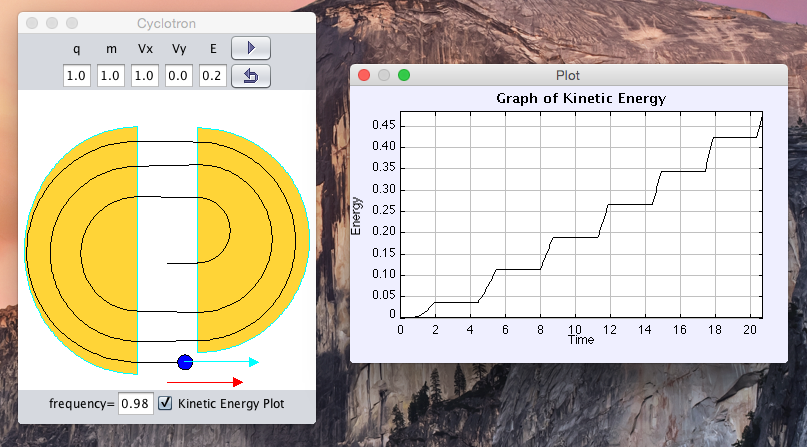
\includegraphics[width=.9\linewidth]{./cycloUI.png}
\caption{UI of the cyclotron experiment}
\end{figure}
\end{itemize} % ends low level

\end{document}
